% Created by tikzDevice version 0.10.1 on 2018-02-18 14:59:26
% !TEX encoding = UTF-8 Unicode
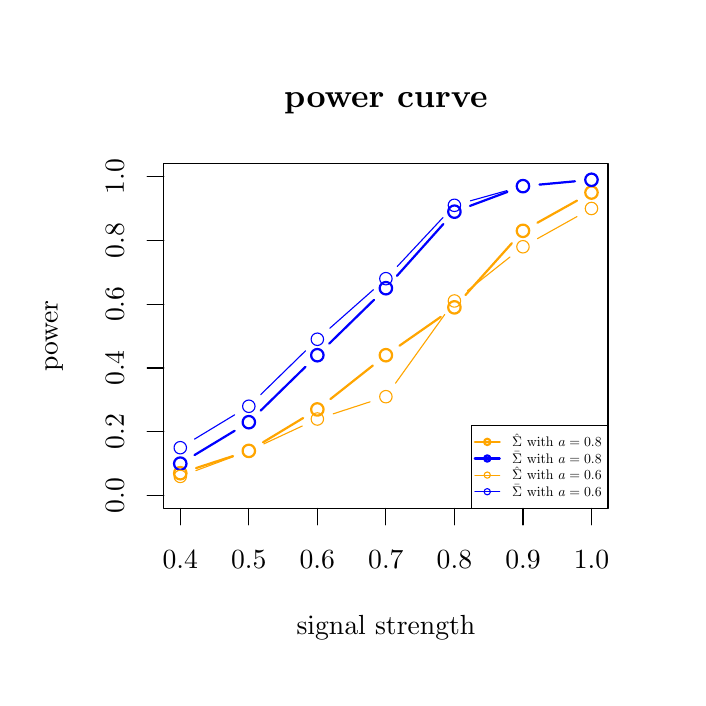
\begin{tikzpicture}[x=1pt,y=1pt]
\definecolor{fillColor}{RGB}{255,255,255}
\path[use as bounding box,fill=fillColor,fill opacity=0.00] (0,0) rectangle (234.88,234.88);
\begin{scope}
\path[clip] ( 49.20, 61.20) rectangle (209.68,185.68);
\definecolor{drawColor}{RGB}{255,165,0}

\path[draw=drawColor,line width= 0.8pt,line join=round,line cap=round] ( 60.85, 75.74) -- ( 74.20, 80.09);

\path[draw=drawColor,line width= 0.8pt,line join=round,line cap=round] ( 85.04, 85.05) -- ( 99.54, 93.82);

\path[draw=drawColor,line width= 0.8pt,line join=round,line cap=round] (109.38,100.65) -- (124.73,112.80);

\path[draw=drawColor,line width= 0.8pt,line join=round,line cap=round] (134.36,119.96) -- (149.28,130.38);

\path[draw=drawColor,line width= 0.8pt,line join=round,line cap=round] (158.21,138.28) -- (174.97,157.00);

\path[draw=drawColor,line width= 0.8pt,line join=round,line cap=round] (184.21,164.40) -- (198.50,172.38);

\path[draw=drawColor,line width= 0.8pt,line join=round,line cap=round] ( 55.14, 73.88) circle (  2.25);

\path[draw=drawColor,line width= 0.8pt,line join=round,line cap=round] ( 79.91, 81.95) circle (  2.25);

\path[draw=drawColor,line width= 0.8pt,line join=round,line cap=round] (104.67, 96.93) circle (  2.25);

\path[draw=drawColor,line width= 0.8pt,line join=round,line cap=round] (129.44,116.52) circle (  2.25);

\path[draw=drawColor,line width= 0.8pt,line join=round,line cap=round] (154.20,133.81) circle (  2.25);

\path[draw=drawColor,line width= 0.8pt,line join=round,line cap=round] (178.97,161.47) circle (  2.25);

\path[draw=drawColor,line width= 0.8pt,line join=round,line cap=round] (203.73,175.30) circle (  2.25);
\end{scope}
\begin{scope}
\path[clip] (  0.00,  0.00) rectangle (234.88,234.88);
\definecolor{drawColor}{RGB}{0,0,0}

\path[draw=drawColor,line width= 0.4pt,line join=round,line cap=round] ( 55.14, 61.20) -- (203.73, 61.20);

\path[draw=drawColor,line width= 0.4pt,line join=round,line cap=round] ( 55.14, 61.20) -- ( 55.14, 55.20);

\path[draw=drawColor,line width= 0.4pt,line join=round,line cap=round] ( 79.91, 61.20) -- ( 79.91, 55.20);

\path[draw=drawColor,line width= 0.4pt,line join=round,line cap=round] (104.67, 61.20) -- (104.67, 55.20);

\path[draw=drawColor,line width= 0.4pt,line join=round,line cap=round] (129.44, 61.20) -- (129.44, 55.20);

\path[draw=drawColor,line width= 0.4pt,line join=round,line cap=round] (154.20, 61.20) -- (154.20, 55.20);

\path[draw=drawColor,line width= 0.4pt,line join=round,line cap=round] (178.97, 61.20) -- (178.97, 55.20);

\path[draw=drawColor,line width= 0.4pt,line join=round,line cap=round] (203.73, 61.20) -- (203.73, 55.20);

\node[text=drawColor,anchor=base,inner sep=0pt, outer sep=0pt, scale=  1.00] at ( 55.14, 39.60) {0.4};

\node[text=drawColor,anchor=base,inner sep=0pt, outer sep=0pt, scale=  1.00] at ( 79.91, 39.60) {0.5};

\node[text=drawColor,anchor=base,inner sep=0pt, outer sep=0pt, scale=  1.00] at (104.67, 39.60) {0.6};

\node[text=drawColor,anchor=base,inner sep=0pt, outer sep=0pt, scale=  1.00] at (129.44, 39.60) {0.7};

\node[text=drawColor,anchor=base,inner sep=0pt, outer sep=0pt, scale=  1.00] at (154.20, 39.60) {0.8};

\node[text=drawColor,anchor=base,inner sep=0pt, outer sep=0pt, scale=  1.00] at (178.97, 39.60) {0.9};

\node[text=drawColor,anchor=base,inner sep=0pt, outer sep=0pt, scale=  1.00] at (203.73, 39.60) {1.0};

\path[draw=drawColor,line width= 0.4pt,line join=round,line cap=round] ( 49.20, 65.81) -- ( 49.20,181.07);

\path[draw=drawColor,line width= 0.4pt,line join=round,line cap=round] ( 49.20, 65.81) -- ( 43.20, 65.81);

\path[draw=drawColor,line width= 0.4pt,line join=round,line cap=round] ( 49.20, 88.86) -- ( 43.20, 88.86);

\path[draw=drawColor,line width= 0.4pt,line join=round,line cap=round] ( 49.20,111.91) -- ( 43.20,111.91);

\path[draw=drawColor,line width= 0.4pt,line join=round,line cap=round] ( 49.20,134.96) -- ( 43.20,134.96);

\path[draw=drawColor,line width= 0.4pt,line join=round,line cap=round] ( 49.20,158.02) -- ( 43.20,158.02);

\path[draw=drawColor,line width= 0.4pt,line join=round,line cap=round] ( 49.20,181.07) -- ( 43.20,181.07);

\node[text=drawColor,rotate= 90.00,anchor=base,inner sep=0pt, outer sep=0pt, scale=  1.00] at ( 34.80, 65.81) {0.0};

\node[text=drawColor,rotate= 90.00,anchor=base,inner sep=0pt, outer sep=0pt, scale=  1.00] at ( 34.80, 88.86) {0.2};

\node[text=drawColor,rotate= 90.00,anchor=base,inner sep=0pt, outer sep=0pt, scale=  1.00] at ( 34.80,111.91) {0.4};

\node[text=drawColor,rotate= 90.00,anchor=base,inner sep=0pt, outer sep=0pt, scale=  1.00] at ( 34.80,134.96) {0.6};

\node[text=drawColor,rotate= 90.00,anchor=base,inner sep=0pt, outer sep=0pt, scale=  1.00] at ( 34.80,158.02) {0.8};

\node[text=drawColor,rotate= 90.00,anchor=base,inner sep=0pt, outer sep=0pt, scale=  1.00] at ( 34.80,181.07) {1.0};

\path[draw=drawColor,line width= 0.4pt,line join=round,line cap=round] ( 49.20, 61.20) --
	(209.68, 61.20) --
	(209.68,185.68) --
	( 49.20,185.68) --
	( 49.20, 61.20);
\end{scope}
\begin{scope}
\path[clip] (  0.00,  0.00) rectangle (234.88,234.88);
\definecolor{drawColor}{RGB}{0,0,0}

\node[text=drawColor,anchor=base,inner sep=0pt, outer sep=0pt, scale=  1.20] at (129.44,206.14) {\bfseries power curve};

\node[text=drawColor,anchor=base,inner sep=0pt, outer sep=0pt, scale=  1.00] at (129.44, 15.60) {signal strength};

\node[text=drawColor,rotate= 90.00,anchor=base,inner sep=0pt, outer sep=0pt, scale=  1.00] at ( 10.80,123.44) {power};
\end{scope}
\begin{scope}
\path[clip] ( 49.20, 61.20) rectangle (209.68,185.68);
\definecolor{drawColor}{RGB}{0,0,255}

\path[draw=drawColor,line width= 0.8pt,line join=round,line cap=round] ( 60.28, 80.44) -- ( 74.78, 89.21);

\path[draw=drawColor,line width= 0.8pt,line join=round,line cap=round] ( 84.20, 96.51) -- (100.38,112.33);

\path[draw=drawColor,line width= 0.8pt,line join=round,line cap=round] (108.96,120.72) -- (125.15,136.53);

\path[draw=drawColor,line width= 0.8pt,line join=round,line cap=round] (133.44,145.20) -- (150.20,163.92);

\path[draw=drawColor,line width= 0.8pt,line join=round,line cap=round] (159.83,170.48) -- (173.35,175.52);

\path[draw=drawColor,line width= 0.8pt,line join=round,line cap=round] (184.94,178.17) -- (197.76,179.36);

\path[draw=drawColor,line width= 0.8pt,line join=round,line cap=round] ( 55.14, 77.34) circle (  2.25);

\path[draw=drawColor,line width= 0.8pt,line join=round,line cap=round] ( 79.91, 92.32) circle (  2.25);

\path[draw=drawColor,line width= 0.8pt,line join=round,line cap=round] (104.67,116.52) circle (  2.25);

\path[draw=drawColor,line width= 0.8pt,line join=round,line cap=round] (129.44,140.73) circle (  2.25);

\path[draw=drawColor,line width= 0.8pt,line join=round,line cap=round] (154.20,168.39) circle (  2.25);

\path[draw=drawColor,line width= 0.8pt,line join=round,line cap=round] (178.97,177.61) circle (  2.25);

\path[draw=drawColor,line width= 0.8pt,line join=round,line cap=round] (203.73,179.91) circle (  2.25);
\definecolor{drawColor}{RGB}{255,165,0}

\path[draw=drawColor,line width= 0.4pt,line join=round,line cap=round] ( 60.77, 74.82) -- ( 74.29, 79.85);

\path[draw=drawColor,line width= 0.4pt,line join=round,line cap=round] ( 85.35, 84.48) -- ( 99.23, 90.94);

\path[draw=drawColor,line width= 0.4pt,line join=round,line cap=round] (110.38, 95.33) -- (123.73, 99.68);

\path[draw=drawColor,line width= 0.4pt,line join=round,line cap=round] (132.93,106.42) -- (150.71,131.24);

\path[draw=drawColor,line width= 0.4pt,line join=round,line cap=round] (158.91,139.84) -- (174.26,151.99);

\path[draw=drawColor,line width= 0.4pt,line join=round,line cap=round] (184.21,158.64) -- (198.50,166.62);

\path[draw=drawColor,line width= 0.4pt,line join=round,line cap=round] ( 55.14, 72.73) circle (  2.25);

\path[draw=drawColor,line width= 0.4pt,line join=round,line cap=round] ( 79.91, 81.95) circle (  2.25);

\path[draw=drawColor,line width= 0.4pt,line join=round,line cap=round] (104.67, 93.47) circle (  2.25);

\path[draw=drawColor,line width= 0.4pt,line join=round,line cap=round] (129.44,101.54) circle (  2.25);

\path[draw=drawColor,line width= 0.4pt,line join=round,line cap=round] (154.20,136.12) circle (  2.25);

\path[draw=drawColor,line width= 0.4pt,line join=round,line cap=round] (178.97,155.71) circle (  2.25);

\path[draw=drawColor,line width= 0.4pt,line join=round,line cap=round] (203.73,169.54) circle (  2.25);
\definecolor{drawColor}{RGB}{0,0,255}

\path[draw=drawColor,line width= 0.4pt,line join=round,line cap=round] ( 60.28, 86.20) -- ( 74.78, 94.98);

\path[draw=drawColor,line width= 0.4pt,line join=round,line cap=round] ( 84.20,102.28) -- (100.38,118.09);

\path[draw=drawColor,line width= 0.4pt,line join=round,line cap=round] (109.17,126.26) -- (124.94,140.21);

\path[draw=drawColor,line width= 0.4pt,line join=round,line cap=round] (133.53,148.57) -- (150.11,166.31);

\path[draw=drawColor,line width= 0.4pt,line join=round,line cap=round] (159.98,172.31) -- (173.19,176.00);

\path[draw=drawColor,line width= 0.4pt,line join=round,line cap=round] (184.94,178.17) -- (197.76,179.36);

\path[draw=drawColor,line width= 0.4pt,line join=round,line cap=round] ( 55.14, 83.10) circle (  2.25);

\path[draw=drawColor,line width= 0.4pt,line join=round,line cap=round] ( 79.91, 98.08) circle (  2.25);

\path[draw=drawColor,line width= 0.4pt,line join=round,line cap=round] (104.67,122.29) circle (  2.25);

\path[draw=drawColor,line width= 0.4pt,line join=round,line cap=round] (129.44,144.18) circle (  2.25);

\path[draw=drawColor,line width= 0.4pt,line join=round,line cap=round] (154.20,170.69) circle (  2.25);

\path[draw=drawColor,line width= 0.4pt,line join=round,line cap=round] (178.97,177.61) circle (  2.25);

\path[draw=drawColor,line width= 0.4pt,line join=round,line cap=round] (203.73,179.91) circle (  2.25);
\definecolor{drawColor}{RGB}{0,0,0}

\path[draw=drawColor,line width= 0.4pt,line join=round,line cap=round] (160.22, 91.20) rectangle (209.68, 61.20);
\definecolor{drawColor}{RGB}{255,165,0}

\path[draw=drawColor,line width= 0.8pt,line join=round,line cap=round] (161.57, 85.20) -- (170.57, 85.20);
\definecolor{drawColor}{RGB}{0,0,255}

\path[draw=drawColor,line width= 0.8pt,line join=round,line cap=round] (161.57, 79.20) -- (170.57, 79.20);
\definecolor{drawColor}{RGB}{255,165,0}

\path[draw=drawColor,line width= 0.4pt,line join=round,line cap=round] (161.57, 73.20) -- (170.57, 73.20);
\definecolor{drawColor}{RGB}{0,0,255}

\path[draw=drawColor,line width= 0.4pt,line join=round,line cap=round] (161.57, 67.20) -- (170.57, 67.20);
\definecolor{drawColor}{RGB}{255,165,0}

\path[draw=drawColor,line width= 0.8pt,line join=round,line cap=round] (166.07, 85.20) circle (  1.13);
\definecolor{drawColor}{RGB}{0,0,255}

\path[draw=drawColor,line width= 0.8pt,line join=round,line cap=round] (166.07, 79.20) circle (  1.13);
\definecolor{drawColor}{RGB}{255,165,0}

\path[draw=drawColor,line width= 0.4pt,line join=round,line cap=round] (166.07, 73.20) circle (  1.13);
\definecolor{drawColor}{RGB}{0,0,255}

\path[draw=drawColor,line width= 0.4pt,line join=round,line cap=round] (166.07, 67.20) circle (  1.13);
\definecolor{drawColor}{RGB}{0,0,0}

\node[text=drawColor,anchor=base west,inner sep=0pt, outer sep=0pt, scale=  0.50] at (175.07, 83.48) {$\hat{\Sigma}$ with $a=0.8$};

\node[text=drawColor,anchor=base west,inner sep=0pt, outer sep=0pt, scale=  0.50] at (175.07, 77.48) {$\bar{\Sigma}$ with $a=0.8$};

\node[text=drawColor,anchor=base west,inner sep=0pt, outer sep=0pt, scale=  0.50] at (175.07, 71.48) {$\hat{\Sigma}$ with $a=0.6$};

\node[text=drawColor,anchor=base west,inner sep=0pt, outer sep=0pt, scale=  0.50] at (175.07, 65.48) {$\bar{\Sigma}$ with $a=0.6$};
\end{scope}
\end{tikzpicture}
